\chapter{Adding sparse point data (own data with geometry)}

\pagestyle{fancy}
\fancyhf{}
\fancyhead[OC]{\leftmark}
\fancyhead[EC]{\rightmark}
%\renewcommand{\footrulewidth}{1pt}
\cfoot{\thepage}


\section{Data}
Filename to use for this section: $headquarters.csv$\\

This file contains our own geographical data regarding the location of the 5 police headquarters. It contains geometry data, as latitude and longitude. QGIS will use this information to plot the data on our map.\\

I created this data file from information I found online. I could only obtain postcode data for the HQ locations. QGIS can not plot postcodes. I needed to do a bit of data processing before can use this in QGIS.  Use free online databases to convert each postcode to either (1) Eastings and Northings, or (2) Latitude and longitude (as required by QGIS to display a point position)\\

\url{https://www.ordnancesurvey.co.uk/business-and-government/products/code-point-open.html}
\url{https://www.freemaptools.com/convert-uk-postcode-to-lat-lng.htm}

\begin{figure}[!h]
	\centering
	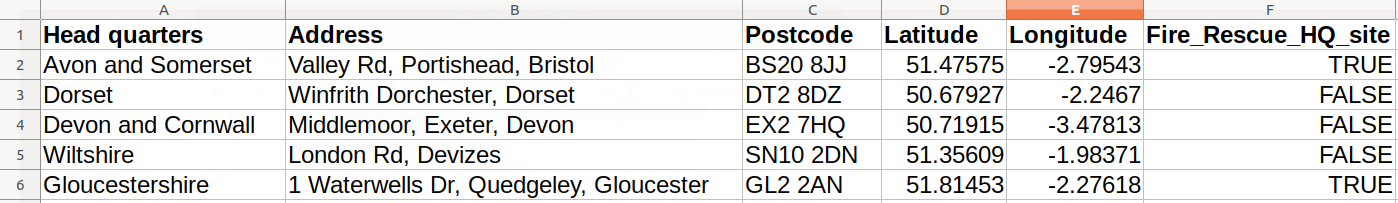
\includegraphics[width=0.8\textwidth]{images/headquarters_csv.png}
	\caption{headquarters.csv file}
	\label{ft_fig_firstfig3}
\end{figure}

\section{Add delimited text file}

Let's add this delimited file 
\begin{tabular}{@{}c@{}}
\includegraphics[width=4ex]{images/add_delimited_text_layer_icon.png}\end{tabular}
.  

Within the \textit{Data Source Manager / Delimited text} window, choose these settings:\\
\textbf{File name:} Navigate to the csv file: $headquarters.csv$\\
\textbf{Layer name} (what appears in the \textit{Layers Panel}, so choose something meaningful): headquarters\\
\textbf{File Format}: CSV (comma separated values)\\
\textbf{Geometry definition} $\rightarrow$ Point coordinates $\rightarrow$  
\textbf{x field} = Longitude \& \textbf{y field} = Latitude\\
\textbf{Coordinate system}: EPSG4326 – WGS 84 (leave as default)\\
(Note: The top row of the csv file is used as the field titles.)\\
\textbf{Add}.\\

\begin{figure}[!h]
	\centering
	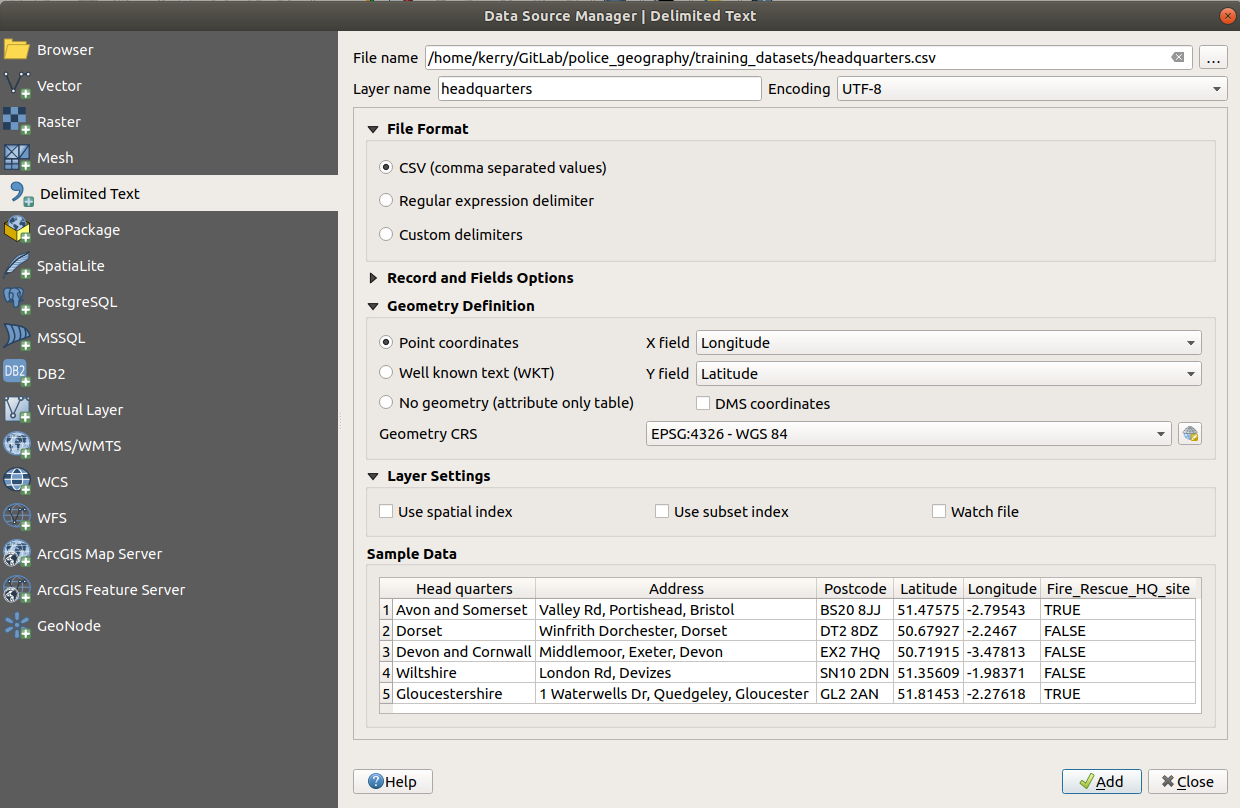
\includegraphics[width=0.8\textwidth]{images/data_source_manager_add_delimited_text.png}
	\caption{Add delimited text file}
	\label{ft_fig_firstfig3}
\end{figure}
\newpage
This new headquarters layer is added to the \emph{layers} panel.\\
The points (with a single symbol) are added to the map canvas.\\
As with all layers, this has it's own attribute table, with a row to represent each point on the map canvas.

If we were keeping the symbol the same for all points we would edit the simple symbol settings in the \emph{Layer styling} panel, by selecting a colour/shape  for the marker to represent the headquarter locations.

%\null\newpage
\begin{figure}[!h]
	\centering
	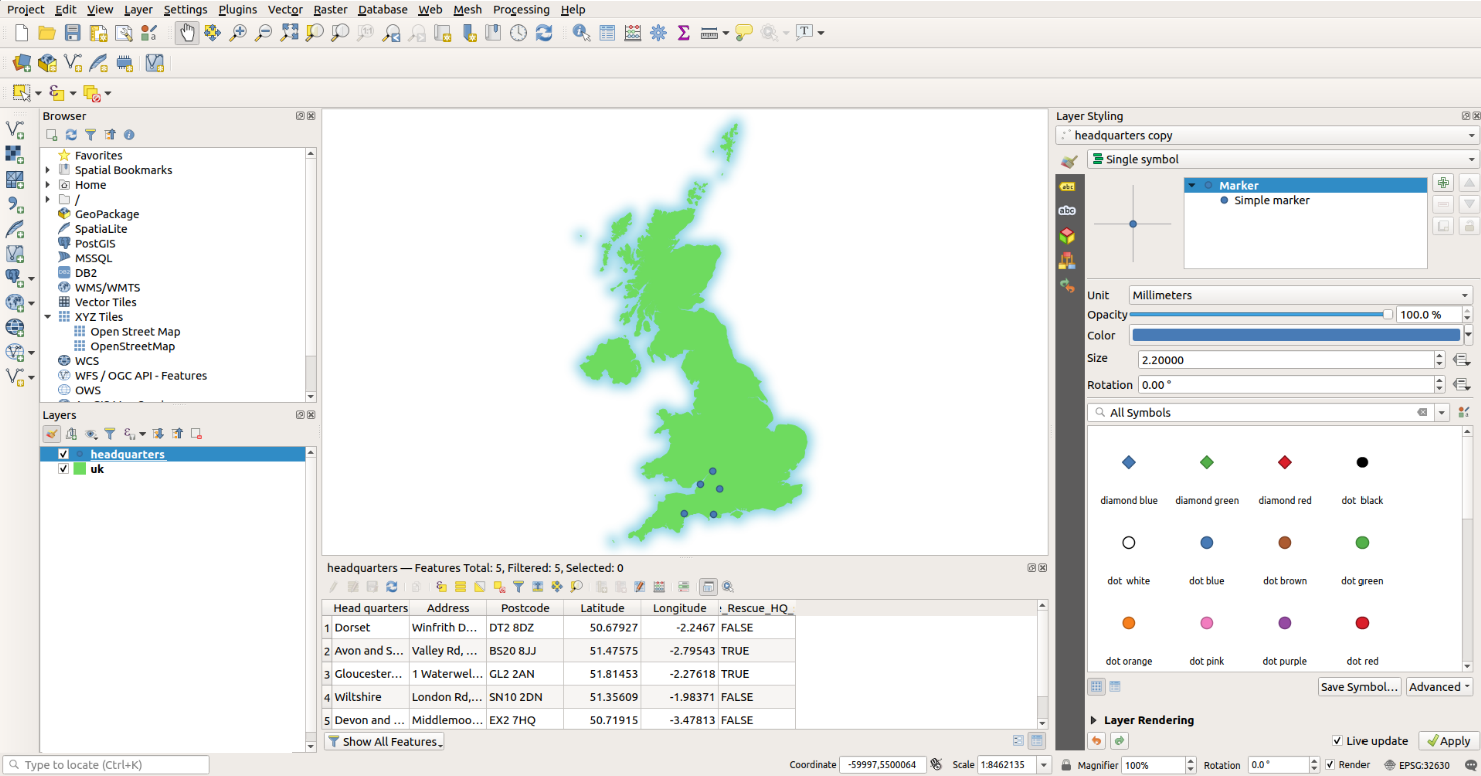
\includegraphics[width=1\textwidth]{images/headquarters_added_to_map.png}
	\caption{headquarters.csv data added to map canvas}
	\label{ft_fig_firstfig3}
\end{figure}



\section{Symbology: Categorized}

We've already explored how to use the \textit{Layers Styling Panel} to change the style of a \textit{Single symbol} (to get the coastline and landmass of UK). Let's now look at how to add different symbol for our points based on a value of a categorical field.\\

This data has a field "Fire\_Rescue\_HQ\_site" which stores a boolean to represent whether the Police HQ location is also the site for the Fire and Rescue HQ. Let's format our points to show this information.\\

In the \textit{Layers Styling Panel}:\\
Select \textit{headquarters}\\
Select \textit{Categorized}\\
\textbf{Column}: Fire\_Rescue\_HQ\_site.  \\
\textbf{Classify}\\

%\begin{figure}[!h]
%	\centering
%	\%includegraphics[width=0.5\textwidth]{images/headquarters_styling1.png}
%	\caption{}
%	\label{ft_fig_firstfig3}
%\end{figure}

Can choose which of the individual categories to be shown on the map (check box next to symbol)\\

\subsection{Choose the style for each symbol} 
To change the shape for all: have nothing highlighted in the pane and select Symbol \begin{tabular}{@{}c@{}}
\includegraphics[width=26ex]{images/symbol_change_button.png}\end{tabular}

To change just one of the symbols: double click an individual symbol.\\

Either have \textit{Marker} highlighted (for one set of symbol options), or select \textit{Simple marker} for more options (explore the options under the different Symbol layer type). It's very easy to get into a pickle here!!\\% Try to change the size and shape.\\

Set legend text to \textit{Police HQ} and \textit{Police \& Fire Rescue HQ}.

%\null\newpage

\begin{figure}[!h]
	\centering
	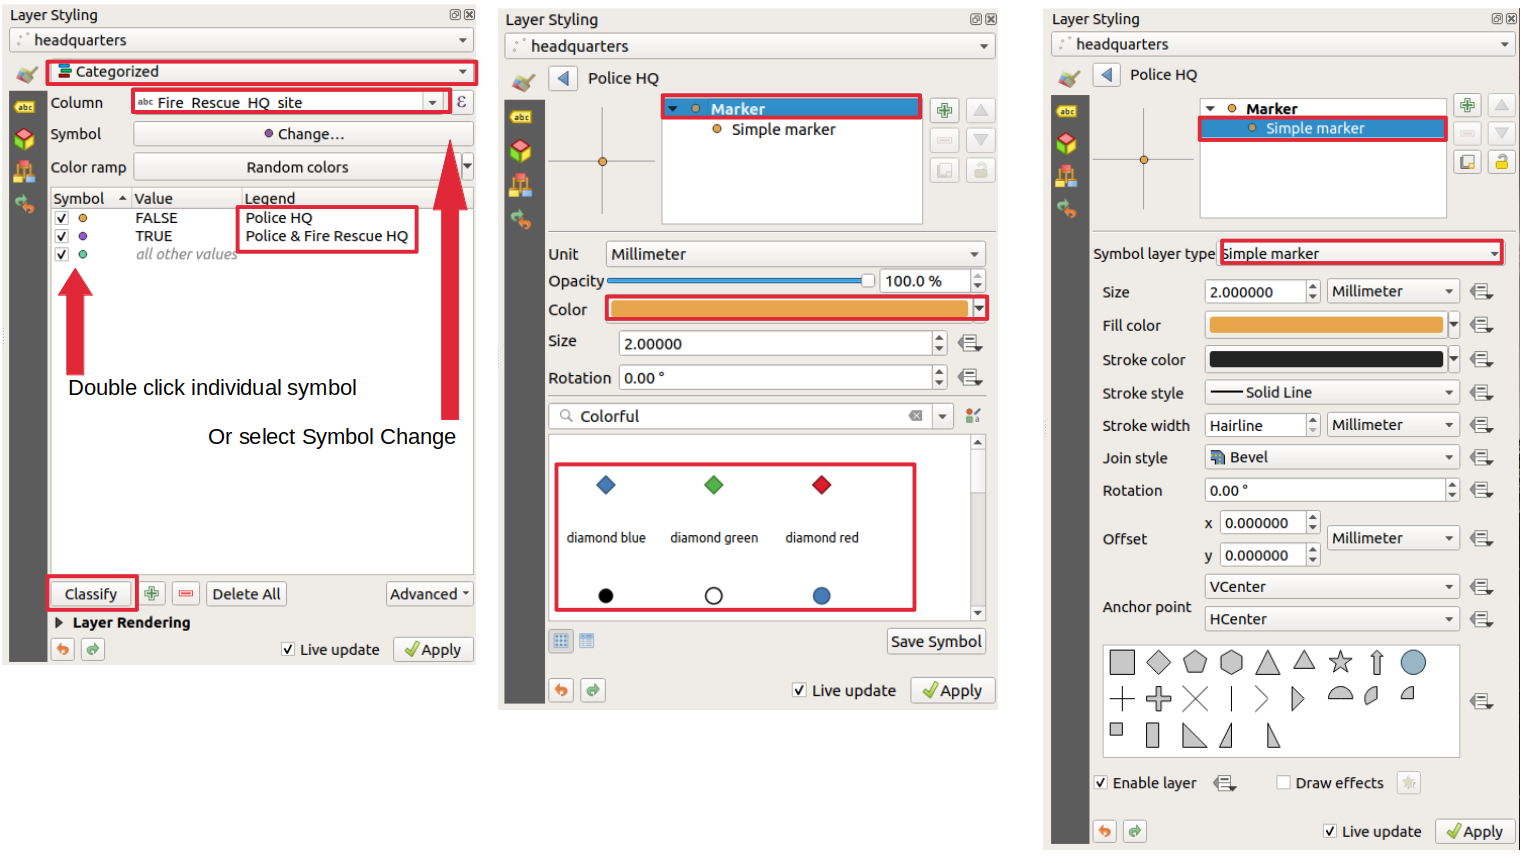
\includegraphics[width=1\textwidth]{images/symbol_symbology.png}%point_data_symbology1.png}
	\caption{How to change symbols for point data using \textit{Layers Styling} panel}
	\label{ft_fig_firstfig3}
\end{figure}

\begin{figure}[!h]
	\centering
	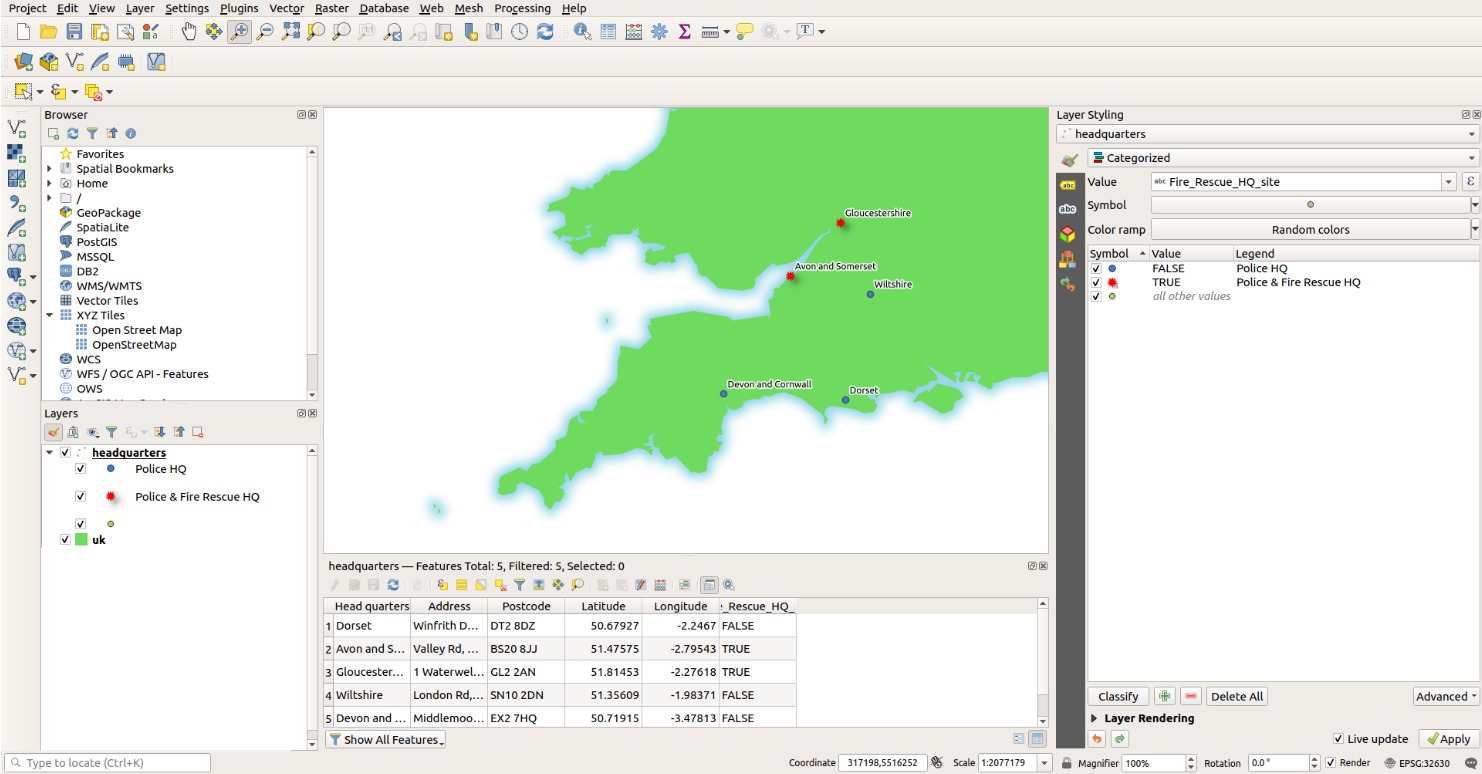
\includegraphics[width=1\textwidth]{images/headquarters_styled.png}
	\caption{headquarters layer with categorized symbology}
	\label{ft_fig_firstfig3}
\end{figure}
\newpage
\subsection{Use rule based styles}

For more complicated allocation of a symbol to field values, can set up rules.

Can see the structure of the rules for the previous styling we chose by selecting “Rule-based”, to edit an existing rule double click on the rule, select the green + button to add a new rule.\\


\begin{figure}[!h]
	\centering
	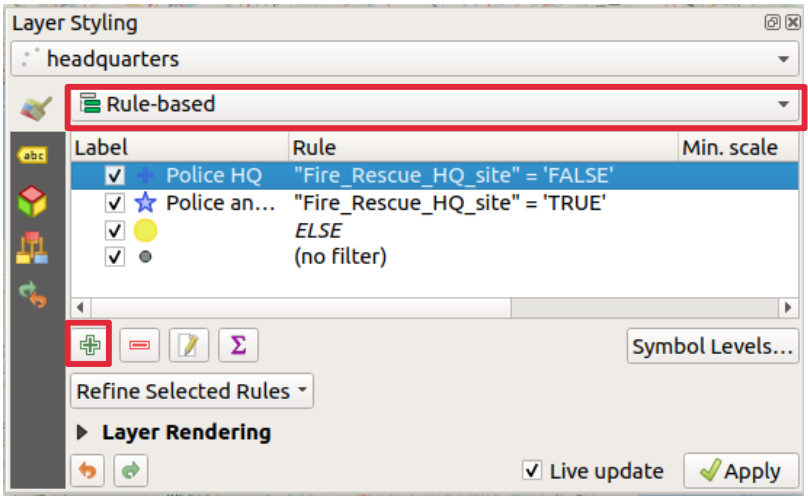
\includegraphics[width=0.5\textwidth]{images/headquarter_rule_based_styles1.png}
	\caption{Rule-based styling}
	\label{ft_fig_firstfig3}
\end{figure}

%
%\begin{figure}[!h]
%	\centering
%	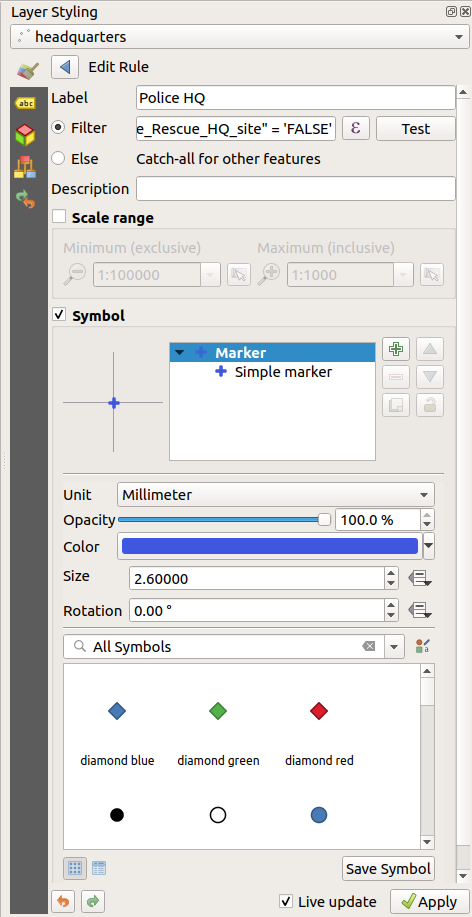
\includegraphics[width=0.3\textwidth]{images/headquarter_rule_based_styles2.png}
%	\caption{}
%	\label{ft_fig_firstfig3}
%\end{figure}

We will set up some rule based labels later, just showing that they are possible for the symbology as well.\\
